% Created by tikzDevice version 0.9 on 2016-01-07 01:19:23
% !TEX encoding = UTF-8 Unicode
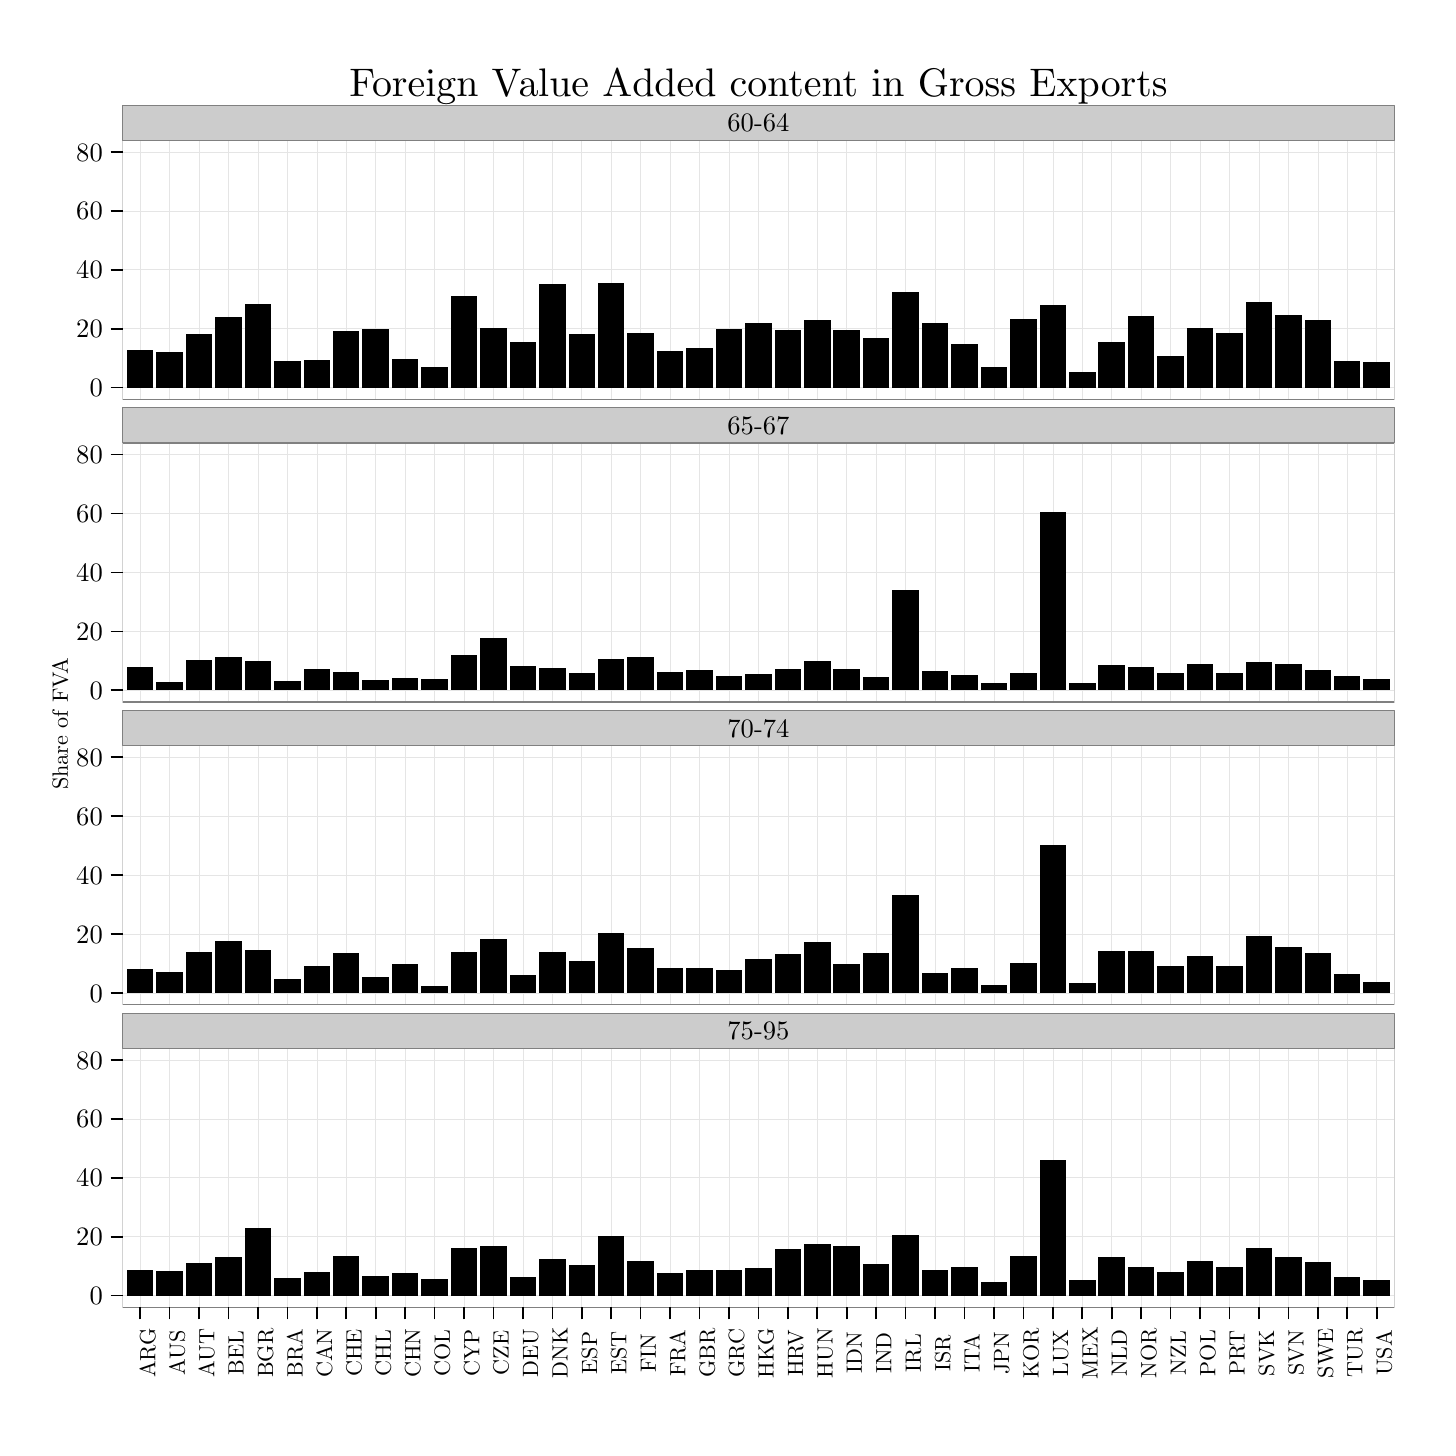
\begin{tikzpicture}[x=1pt,y=1pt]
\definecolor{fillColor}{RGB}{255,255,255}
\path[use as bounding box,fill=fillColor,fill opacity=0.00] (0,0) rectangle (505.89,505.89);
\begin{scope}
\path[clip] (  0.00,  0.00) rectangle (505.89,505.89);
\definecolor{drawColor}{RGB}{255,255,255}
\definecolor{fillColor}{RGB}{255,255,255}

\path[draw=drawColor,line width= 0.6pt,line join=round,line cap=round,fill=fillColor] (  0.00,  0.00) rectangle (505.89,505.89);
\end{scope}
\begin{scope}
\path[clip] ( 34.27,371.55) rectangle (493.85,465.27);
\definecolor{fillColor}{RGB}{255,255,255}

\path[fill=fillColor] ( 34.27,371.55) rectangle (493.85,465.27);
\definecolor{drawColor}{gray}{0.90}

\path[draw=drawColor,line width= 0.2pt,line join=round] ( 34.27,375.81) --
	(493.85,375.81);

\path[draw=drawColor,line width= 0.2pt,line join=round] ( 34.27,397.11) --
	(493.85,397.11);

\path[draw=drawColor,line width= 0.2pt,line join=round] ( 34.27,418.41) --
	(493.85,418.41);

\path[draw=drawColor,line width= 0.2pt,line join=round] ( 34.27,439.71) --
	(493.85,439.71);

\path[draw=drawColor,line width= 0.2pt,line join=round] ( 34.27,461.01) --
	(493.85,461.01);

\path[draw=drawColor,line width= 0.2pt,line join=round] ( 40.65,371.55) --
	( 40.65,465.27);

\path[draw=drawColor,line width= 0.2pt,line join=round] ( 51.29,371.55) --
	( 51.29,465.27);

\path[draw=drawColor,line width= 0.2pt,line join=round] ( 61.93,371.55) --
	( 61.93,465.27);

\path[draw=drawColor,line width= 0.2pt,line join=round] ( 72.56,371.55) --
	( 72.56,465.27);

\path[draw=drawColor,line width= 0.2pt,line join=round] ( 83.20,371.55) --
	( 83.20,465.27);

\path[draw=drawColor,line width= 0.2pt,line join=round] ( 93.84,371.55) --
	( 93.84,465.27);

\path[draw=drawColor,line width= 0.2pt,line join=round] (104.48,371.55) --
	(104.48,465.27);

\path[draw=drawColor,line width= 0.2pt,line join=round] (115.12,371.55) --
	(115.12,465.27);

\path[draw=drawColor,line width= 0.2pt,line join=round] (125.76,371.55) --
	(125.76,465.27);

\path[draw=drawColor,line width= 0.2pt,line join=round] (136.39,371.55) --
	(136.39,465.27);

\path[draw=drawColor,line width= 0.2pt,line join=round] (147.03,371.55) --
	(147.03,465.27);

\path[draw=drawColor,line width= 0.2pt,line join=round] (157.67,371.55) --
	(157.67,465.27);

\path[draw=drawColor,line width= 0.2pt,line join=round] (168.31,371.55) --
	(168.31,465.27);

\path[draw=drawColor,line width= 0.2pt,line join=round] (178.95,371.55) --
	(178.95,465.27);

\path[draw=drawColor,line width= 0.2pt,line join=round] (189.59,371.55) --
	(189.59,465.27);

\path[draw=drawColor,line width= 0.2pt,line join=round] (200.22,371.55) --
	(200.22,465.27);

\path[draw=drawColor,line width= 0.2pt,line join=round] (210.86,371.55) --
	(210.86,465.27);

\path[draw=drawColor,line width= 0.2pt,line join=round] (221.50,371.55) --
	(221.50,465.27);

\path[draw=drawColor,line width= 0.2pt,line join=round] (232.14,371.55) --
	(232.14,465.27);

\path[draw=drawColor,line width= 0.2pt,line join=round] (242.78,371.55) --
	(242.78,465.27);

\path[draw=drawColor,line width= 0.2pt,line join=round] (253.42,371.55) --
	(253.42,465.27);

\path[draw=drawColor,line width= 0.2pt,line join=round] (264.06,371.55) --
	(264.06,465.27);

\path[draw=drawColor,line width= 0.2pt,line join=round] (274.69,371.55) --
	(274.69,465.27);

\path[draw=drawColor,line width= 0.2pt,line join=round] (285.33,371.55) --
	(285.33,465.27);

\path[draw=drawColor,line width= 0.2pt,line join=round] (295.97,371.55) --
	(295.97,465.27);

\path[draw=drawColor,line width= 0.2pt,line join=round] (306.61,371.55) --
	(306.61,465.27);

\path[draw=drawColor,line width= 0.2pt,line join=round] (317.25,371.55) --
	(317.25,465.27);

\path[draw=drawColor,line width= 0.2pt,line join=round] (327.89,371.55) --
	(327.89,465.27);

\path[draw=drawColor,line width= 0.2pt,line join=round] (338.52,371.55) --
	(338.52,465.27);

\path[draw=drawColor,line width= 0.2pt,line join=round] (349.16,371.55) --
	(349.16,465.27);

\path[draw=drawColor,line width= 0.2pt,line join=round] (359.80,371.55) --
	(359.80,465.27);

\path[draw=drawColor,line width= 0.2pt,line join=round] (370.44,371.55) --
	(370.44,465.27);

\path[draw=drawColor,line width= 0.2pt,line join=round] (381.08,371.55) --
	(381.08,465.27);

\path[draw=drawColor,line width= 0.2pt,line join=round] (391.72,371.55) --
	(391.72,465.27);

\path[draw=drawColor,line width= 0.2pt,line join=round] (402.35,371.55) --
	(402.35,465.27);

\path[draw=drawColor,line width= 0.2pt,line join=round] (412.99,371.55) --
	(412.99,465.27);

\path[draw=drawColor,line width= 0.2pt,line join=round] (423.63,371.55) --
	(423.63,465.27);

\path[draw=drawColor,line width= 0.2pt,line join=round] (434.27,371.55) --
	(434.27,465.27);

\path[draw=drawColor,line width= 0.2pt,line join=round] (444.91,371.55) --
	(444.91,465.27);

\path[draw=drawColor,line width= 0.2pt,line join=round] (455.55,371.55) --
	(455.55,465.27);

\path[draw=drawColor,line width= 0.2pt,line join=round] (466.19,371.55) --
	(466.19,465.27);

\path[draw=drawColor,line width= 0.2pt,line join=round] (476.82,371.55) --
	(476.82,465.27);

\path[draw=drawColor,line width= 0.2pt,line join=round] (487.46,371.55) --
	(487.46,465.27);
\definecolor{fillColor}{RGB}{0,0,0}

\path[fill=fillColor] ( 35.86,375.81) rectangle ( 45.44,389.47);

\path[fill=fillColor] ( 46.50,375.81) rectangle ( 56.07,388.84);

\path[fill=fillColor] ( 57.14,375.81) rectangle ( 66.71,395.08);

\path[fill=fillColor] ( 67.78,375.81) rectangle ( 77.35,401.32);

\path[fill=fillColor] ( 78.42,375.81) rectangle ( 87.99,406.18);

\path[fill=fillColor] ( 89.05,375.81) rectangle ( 98.63,385.31);

\path[fill=fillColor] ( 99.69,375.81) rectangle (109.27,385.95);

\path[fill=fillColor] (110.33,375.81) rectangle (119.90,396.18);

\path[fill=fillColor] (120.97,375.81) rectangle (130.54,396.85);

\path[fill=fillColor] (131.61,375.81) rectangle (141.18,386.22);

\path[fill=fillColor] (142.25,375.81) rectangle (151.82,383.39);

\path[fill=fillColor] (152.88,375.81) rectangle (162.46,409.04);

\path[fill=fillColor] (163.52,375.81) rectangle (173.10,397.43);

\path[fill=fillColor] (174.16,375.81) rectangle (183.74,392.30);

\path[fill=fillColor] (184.80,375.81) rectangle (194.37,413.19);

\path[fill=fillColor] (195.44,375.81) rectangle (205.01,395.08);

\path[fill=fillColor] (206.08,375.81) rectangle (215.65,413.77);

\path[fill=fillColor] (216.71,375.81) rectangle (226.29,395.44);

\path[fill=fillColor] (227.35,375.81) rectangle (236.93,389.16);

\path[fill=fillColor] (237.99,375.81) rectangle (247.57,389.98);

\path[fill=fillColor] (248.63,375.81) rectangle (258.20,397.01);

\path[fill=fillColor] (259.27,375.81) rectangle (268.84,399.05);

\path[fill=fillColor] (269.91,375.81) rectangle (279.48,396.59);

\path[fill=fillColor] (280.54,375.81) rectangle (290.12,400.08);

\path[fill=fillColor] (291.18,375.81) rectangle (300.76,396.67);

\path[fill=fillColor] (301.82,375.81) rectangle (311.40,393.69);

\path[fill=fillColor] (312.46,375.81) rectangle (322.03,410.22);

\path[fill=fillColor] (323.10,375.81) rectangle (332.67,399.26);

\path[fill=fillColor] (333.74,375.81) rectangle (343.31,391.52);

\path[fill=fillColor] (344.38,375.81) rectangle (353.95,383.23);

\path[fill=fillColor] (355.01,375.81) rectangle (364.59,400.54);

\path[fill=fillColor] (365.65,375.81) rectangle (375.23,405.64);

\path[fill=fillColor] (376.29,375.81) rectangle (385.87,381.40);

\path[fill=fillColor] (386.93,375.81) rectangle (396.50,392.43);

\path[fill=fillColor] (397.57,375.81) rectangle (407.14,401.77);

\path[fill=fillColor] (408.21,375.81) rectangle (417.78,387.28);

\path[fill=fillColor] (418.84,375.81) rectangle (428.42,397.54);

\path[fill=fillColor] (429.48,375.81) rectangle (439.06,395.39);

\path[fill=fillColor] (440.12,375.81) rectangle (449.70,406.82);

\path[fill=fillColor] (450.76,375.81) rectangle (460.33,402.15);

\path[fill=fillColor] (461.40,375.81) rectangle (470.97,400.09);

\path[fill=fillColor] (472.04,375.81) rectangle (481.61,385.33);

\path[fill=fillColor] (482.67,375.81) rectangle (492.25,385.03);
\definecolor{drawColor}{gray}{0.50}

\path[draw=drawColor,line width= 0.6pt,line join=round,line cap=round] ( 34.27,371.55) rectangle (493.85,465.27);
\end{scope}
\begin{scope}
\path[clip] ( 34.27,262.18) rectangle (493.85,355.90);
\definecolor{fillColor}{RGB}{255,255,255}

\path[fill=fillColor] ( 34.27,262.18) rectangle (493.85,355.90);
\definecolor{drawColor}{gray}{0.90}

\path[draw=drawColor,line width= 0.2pt,line join=round] ( 34.27,266.44) --
	(493.85,266.44);

\path[draw=drawColor,line width= 0.2pt,line join=round] ( 34.27,287.74) --
	(493.85,287.74);

\path[draw=drawColor,line width= 0.2pt,line join=round] ( 34.27,309.04) --
	(493.85,309.04);

\path[draw=drawColor,line width= 0.2pt,line join=round] ( 34.27,330.34) --
	(493.85,330.34);

\path[draw=drawColor,line width= 0.2pt,line join=round] ( 34.27,351.64) --
	(493.85,351.64);

\path[draw=drawColor,line width= 0.2pt,line join=round] ( 40.65,262.18) --
	( 40.65,355.90);

\path[draw=drawColor,line width= 0.2pt,line join=round] ( 51.29,262.18) --
	( 51.29,355.90);

\path[draw=drawColor,line width= 0.2pt,line join=round] ( 61.93,262.18) --
	( 61.93,355.90);

\path[draw=drawColor,line width= 0.2pt,line join=round] ( 72.56,262.18) --
	( 72.56,355.90);

\path[draw=drawColor,line width= 0.2pt,line join=round] ( 83.20,262.18) --
	( 83.20,355.90);

\path[draw=drawColor,line width= 0.2pt,line join=round] ( 93.84,262.18) --
	( 93.84,355.90);

\path[draw=drawColor,line width= 0.2pt,line join=round] (104.48,262.18) --
	(104.48,355.90);

\path[draw=drawColor,line width= 0.2pt,line join=round] (115.12,262.18) --
	(115.12,355.90);

\path[draw=drawColor,line width= 0.2pt,line join=round] (125.76,262.18) --
	(125.76,355.90);

\path[draw=drawColor,line width= 0.2pt,line join=round] (136.39,262.18) --
	(136.39,355.90);

\path[draw=drawColor,line width= 0.2pt,line join=round] (147.03,262.18) --
	(147.03,355.90);

\path[draw=drawColor,line width= 0.2pt,line join=round] (157.67,262.18) --
	(157.67,355.90);

\path[draw=drawColor,line width= 0.2pt,line join=round] (168.31,262.18) --
	(168.31,355.90);

\path[draw=drawColor,line width= 0.2pt,line join=round] (178.95,262.18) --
	(178.95,355.90);

\path[draw=drawColor,line width= 0.2pt,line join=round] (189.59,262.18) --
	(189.59,355.90);

\path[draw=drawColor,line width= 0.2pt,line join=round] (200.22,262.18) --
	(200.22,355.90);

\path[draw=drawColor,line width= 0.2pt,line join=round] (210.86,262.18) --
	(210.86,355.90);

\path[draw=drawColor,line width= 0.2pt,line join=round] (221.50,262.18) --
	(221.50,355.90);

\path[draw=drawColor,line width= 0.2pt,line join=round] (232.14,262.18) --
	(232.14,355.90);

\path[draw=drawColor,line width= 0.2pt,line join=round] (242.78,262.18) --
	(242.78,355.90);

\path[draw=drawColor,line width= 0.2pt,line join=round] (253.42,262.18) --
	(253.42,355.90);

\path[draw=drawColor,line width= 0.2pt,line join=round] (264.06,262.18) --
	(264.06,355.90);

\path[draw=drawColor,line width= 0.2pt,line join=round] (274.69,262.18) --
	(274.69,355.90);

\path[draw=drawColor,line width= 0.2pt,line join=round] (285.33,262.18) --
	(285.33,355.90);

\path[draw=drawColor,line width= 0.2pt,line join=round] (295.97,262.18) --
	(295.97,355.90);

\path[draw=drawColor,line width= 0.2pt,line join=round] (306.61,262.18) --
	(306.61,355.90);

\path[draw=drawColor,line width= 0.2pt,line join=round] (317.25,262.18) --
	(317.25,355.90);

\path[draw=drawColor,line width= 0.2pt,line join=round] (327.89,262.18) --
	(327.89,355.90);

\path[draw=drawColor,line width= 0.2pt,line join=round] (338.52,262.18) --
	(338.52,355.90);

\path[draw=drawColor,line width= 0.2pt,line join=round] (349.16,262.18) --
	(349.16,355.90);

\path[draw=drawColor,line width= 0.2pt,line join=round] (359.80,262.18) --
	(359.80,355.90);

\path[draw=drawColor,line width= 0.2pt,line join=round] (370.44,262.18) --
	(370.44,355.90);

\path[draw=drawColor,line width= 0.2pt,line join=round] (381.08,262.18) --
	(381.08,355.90);

\path[draw=drawColor,line width= 0.2pt,line join=round] (391.72,262.18) --
	(391.72,355.90);

\path[draw=drawColor,line width= 0.2pt,line join=round] (402.35,262.18) --
	(402.35,355.90);

\path[draw=drawColor,line width= 0.2pt,line join=round] (412.99,262.18) --
	(412.99,355.90);

\path[draw=drawColor,line width= 0.2pt,line join=round] (423.63,262.18) --
	(423.63,355.90);

\path[draw=drawColor,line width= 0.2pt,line join=round] (434.27,262.18) --
	(434.27,355.90);

\path[draw=drawColor,line width= 0.2pt,line join=round] (444.91,262.18) --
	(444.91,355.90);

\path[draw=drawColor,line width= 0.2pt,line join=round] (455.55,262.18) --
	(455.55,355.90);

\path[draw=drawColor,line width= 0.2pt,line join=round] (466.19,262.18) --
	(466.19,355.90);

\path[draw=drawColor,line width= 0.2pt,line join=round] (476.82,262.18) --
	(476.82,355.90);

\path[draw=drawColor,line width= 0.2pt,line join=round] (487.46,262.18) --
	(487.46,355.90);
\definecolor{fillColor}{RGB}{0,0,0}

\path[fill=fillColor] ( 35.86,266.44) rectangle ( 45.44,274.74);

\path[fill=fillColor] ( 46.50,266.44) rectangle ( 56.07,269.46);

\path[fill=fillColor] ( 57.14,266.44) rectangle ( 66.71,277.48);

\path[fill=fillColor] ( 67.78,266.44) rectangle ( 77.35,278.37);

\path[fill=fillColor] ( 78.42,266.44) rectangle ( 87.99,276.98);

\path[fill=fillColor] ( 89.05,266.44) rectangle ( 98.63,269.76);

\path[fill=fillColor] ( 99.69,266.44) rectangle (109.27,274.09);

\path[fill=fillColor] (110.33,266.44) rectangle (119.90,272.90);

\path[fill=fillColor] (120.97,266.44) rectangle (130.54,270.32);

\path[fill=fillColor] (131.61,266.44) rectangle (141.18,270.85);

\path[fill=fillColor] (142.25,266.44) rectangle (151.82,270.57);

\path[fill=fillColor] (152.88,266.44) rectangle (162.46,279.16);

\path[fill=fillColor] (163.52,266.44) rectangle (173.10,285.44);

\path[fill=fillColor] (174.16,266.44) rectangle (183.74,275.19);

\path[fill=fillColor] (184.80,266.44) rectangle (194.37,274.47);

\path[fill=fillColor] (195.44,266.44) rectangle (205.01,272.87);

\path[fill=fillColor] (206.08,266.44) rectangle (215.65,277.66);

\path[fill=fillColor] (216.71,266.44) rectangle (226.29,278.64);

\path[fill=fillColor] (227.35,266.44) rectangle (236.93,273.07);

\path[fill=fillColor] (237.99,266.44) rectangle (247.57,273.81);

\path[fill=fillColor] (248.63,266.44) rectangle (258.20,271.68);

\path[fill=fillColor] (259.27,266.44) rectangle (268.84,272.45);

\path[fill=fillColor] (269.91,266.44) rectangle (279.48,273.98);

\path[fill=fillColor] (280.54,266.44) rectangle (290.12,277.11);

\path[fill=fillColor] (291.18,266.44) rectangle (300.76,274.03);

\path[fill=fillColor] (301.82,266.44) rectangle (311.40,271.40);

\path[fill=fillColor] (312.46,266.44) rectangle (322.03,302.77);

\path[fill=fillColor] (323.10,266.44) rectangle (332.67,273.30);

\path[fill=fillColor] (333.74,266.44) rectangle (343.31,271.95);

\path[fill=fillColor] (344.38,266.44) rectangle (353.95,268.99);

\path[fill=fillColor] (355.01,266.44) rectangle (364.59,272.68);

\path[fill=fillColor] (365.65,266.44) rectangle (375.23,330.71);

\path[fill=fillColor] (376.29,266.44) rectangle (385.87,268.97);

\path[fill=fillColor] (386.93,266.44) rectangle (396.50,275.58);

\path[fill=fillColor] (397.57,266.44) rectangle (407.14,274.99);

\path[fill=fillColor] (408.21,266.44) rectangle (417.78,272.74);

\path[fill=fillColor] (418.84,266.44) rectangle (428.42,276.09);

\path[fill=fillColor] (429.48,266.44) rectangle (439.06,272.68);

\path[fill=fillColor] (440.12,266.44) rectangle (449.70,276.83);

\path[fill=fillColor] (450.76,266.44) rectangle (460.33,275.98);

\path[fill=fillColor] (461.40,266.44) rectangle (470.97,273.65);

\path[fill=fillColor] (472.04,266.44) rectangle (481.61,271.71);

\path[fill=fillColor] (482.67,266.44) rectangle (492.25,270.42);
\definecolor{drawColor}{gray}{0.50}

\path[draw=drawColor,line width= 0.6pt,line join=round,line cap=round] ( 34.27,262.18) rectangle (493.85,355.90);
\end{scope}
\begin{scope}
\path[clip] ( 34.27,152.81) rectangle (493.85,246.53);
\definecolor{fillColor}{RGB}{255,255,255}

\path[fill=fillColor] ( 34.27,152.81) rectangle (493.85,246.53);
\definecolor{drawColor}{gray}{0.90}

\path[draw=drawColor,line width= 0.2pt,line join=round] ( 34.27,157.07) --
	(493.85,157.07);

\path[draw=drawColor,line width= 0.2pt,line join=round] ( 34.27,178.37) --
	(493.85,178.37);

\path[draw=drawColor,line width= 0.2pt,line join=round] ( 34.27,199.67) --
	(493.85,199.67);

\path[draw=drawColor,line width= 0.2pt,line join=round] ( 34.27,220.97) --
	(493.85,220.97);

\path[draw=drawColor,line width= 0.2pt,line join=round] ( 34.27,242.27) --
	(493.85,242.27);

\path[draw=drawColor,line width= 0.2pt,line join=round] ( 40.65,152.81) --
	( 40.65,246.53);

\path[draw=drawColor,line width= 0.2pt,line join=round] ( 51.29,152.81) --
	( 51.29,246.53);

\path[draw=drawColor,line width= 0.2pt,line join=round] ( 61.93,152.81) --
	( 61.93,246.53);

\path[draw=drawColor,line width= 0.2pt,line join=round] ( 72.56,152.81) --
	( 72.56,246.53);

\path[draw=drawColor,line width= 0.2pt,line join=round] ( 83.20,152.81) --
	( 83.20,246.53);

\path[draw=drawColor,line width= 0.2pt,line join=round] ( 93.84,152.81) --
	( 93.84,246.53);

\path[draw=drawColor,line width= 0.2pt,line join=round] (104.48,152.81) --
	(104.48,246.53);

\path[draw=drawColor,line width= 0.2pt,line join=round] (115.12,152.81) --
	(115.12,246.53);

\path[draw=drawColor,line width= 0.2pt,line join=round] (125.76,152.81) --
	(125.76,246.53);

\path[draw=drawColor,line width= 0.2pt,line join=round] (136.39,152.81) --
	(136.39,246.53);

\path[draw=drawColor,line width= 0.2pt,line join=round] (147.03,152.81) --
	(147.03,246.53);

\path[draw=drawColor,line width= 0.2pt,line join=round] (157.67,152.81) --
	(157.67,246.53);

\path[draw=drawColor,line width= 0.2pt,line join=round] (168.31,152.81) --
	(168.31,246.53);

\path[draw=drawColor,line width= 0.2pt,line join=round] (178.95,152.81) --
	(178.95,246.53);

\path[draw=drawColor,line width= 0.2pt,line join=round] (189.59,152.81) --
	(189.59,246.53);

\path[draw=drawColor,line width= 0.2pt,line join=round] (200.22,152.81) --
	(200.22,246.53);

\path[draw=drawColor,line width= 0.2pt,line join=round] (210.86,152.81) --
	(210.86,246.53);

\path[draw=drawColor,line width= 0.2pt,line join=round] (221.50,152.81) --
	(221.50,246.53);

\path[draw=drawColor,line width= 0.2pt,line join=round] (232.14,152.81) --
	(232.14,246.53);

\path[draw=drawColor,line width= 0.2pt,line join=round] (242.78,152.81) --
	(242.78,246.53);

\path[draw=drawColor,line width= 0.2pt,line join=round] (253.42,152.81) --
	(253.42,246.53);

\path[draw=drawColor,line width= 0.2pt,line join=round] (264.06,152.81) --
	(264.06,246.53);

\path[draw=drawColor,line width= 0.2pt,line join=round] (274.69,152.81) --
	(274.69,246.53);

\path[draw=drawColor,line width= 0.2pt,line join=round] (285.33,152.81) --
	(285.33,246.53);

\path[draw=drawColor,line width= 0.2pt,line join=round] (295.97,152.81) --
	(295.97,246.53);

\path[draw=drawColor,line width= 0.2pt,line join=round] (306.61,152.81) --
	(306.61,246.53);

\path[draw=drawColor,line width= 0.2pt,line join=round] (317.25,152.81) --
	(317.25,246.53);

\path[draw=drawColor,line width= 0.2pt,line join=round] (327.89,152.81) --
	(327.89,246.53);

\path[draw=drawColor,line width= 0.2pt,line join=round] (338.52,152.81) --
	(338.52,246.53);

\path[draw=drawColor,line width= 0.2pt,line join=round] (349.16,152.81) --
	(349.16,246.53);

\path[draw=drawColor,line width= 0.2pt,line join=round] (359.80,152.81) --
	(359.80,246.53);

\path[draw=drawColor,line width= 0.2pt,line join=round] (370.44,152.81) --
	(370.44,246.53);

\path[draw=drawColor,line width= 0.2pt,line join=round] (381.08,152.81) --
	(381.08,246.53);

\path[draw=drawColor,line width= 0.2pt,line join=round] (391.72,152.81) --
	(391.72,246.53);

\path[draw=drawColor,line width= 0.2pt,line join=round] (402.35,152.81) --
	(402.35,246.53);

\path[draw=drawColor,line width= 0.2pt,line join=round] (412.99,152.81) --
	(412.99,246.53);

\path[draw=drawColor,line width= 0.2pt,line join=round] (423.63,152.81) --
	(423.63,246.53);

\path[draw=drawColor,line width= 0.2pt,line join=round] (434.27,152.81) --
	(434.27,246.53);

\path[draw=drawColor,line width= 0.2pt,line join=round] (444.91,152.81) --
	(444.91,246.53);

\path[draw=drawColor,line width= 0.2pt,line join=round] (455.55,152.81) --
	(455.55,246.53);

\path[draw=drawColor,line width= 0.2pt,line join=round] (466.19,152.81) --
	(466.19,246.53);

\path[draw=drawColor,line width= 0.2pt,line join=round] (476.82,152.81) --
	(476.82,246.53);

\path[draw=drawColor,line width= 0.2pt,line join=round] (487.46,152.81) --
	(487.46,246.53);
\definecolor{fillColor}{RGB}{0,0,0}

\path[fill=fillColor] ( 35.86,157.07) rectangle ( 45.44,165.62);

\path[fill=fillColor] ( 46.50,157.07) rectangle ( 56.07,164.53);

\path[fill=fillColor] ( 57.14,157.07) rectangle ( 66.71,171.73);

\path[fill=fillColor] ( 67.78,157.07) rectangle ( 77.35,175.97);

\path[fill=fillColor] ( 78.42,157.07) rectangle ( 87.99,172.78);

\path[fill=fillColor] ( 89.05,157.07) rectangle ( 98.63,162.01);

\path[fill=fillColor] ( 99.69,157.07) rectangle (109.27,166.74);

\path[fill=fillColor] (110.33,157.07) rectangle (119.90,171.37);

\path[fill=fillColor] (120.97,157.07) rectangle (130.54,162.81);

\path[fill=fillColor] (131.61,157.07) rectangle (141.18,167.72);

\path[fill=fillColor] (142.25,157.07) rectangle (151.82,159.72);

\path[fill=fillColor] (152.88,157.07) rectangle (162.46,171.78);

\path[fill=fillColor] (163.52,157.07) rectangle (173.10,176.74);

\path[fill=fillColor] (174.16,157.07) rectangle (183.74,163.65);

\path[fill=fillColor] (184.80,157.07) rectangle (194.37,171.91);

\path[fill=fillColor] (195.44,157.07) rectangle (205.01,168.53);

\path[fill=fillColor] (206.08,157.07) rectangle (215.65,178.62);

\path[fill=fillColor] (216.71,157.07) rectangle (226.29,173.46);

\path[fill=fillColor] (227.35,157.07) rectangle (236.93,166.00);

\path[fill=fillColor] (237.99,157.07) rectangle (247.57,166.15);

\path[fill=fillColor] (248.63,157.07) rectangle (258.20,165.52);

\path[fill=fillColor] (259.27,157.07) rectangle (268.84,169.53);

\path[fill=fillColor] (269.91,157.07) rectangle (279.48,171.17);

\path[fill=fillColor] (280.54,157.07) rectangle (290.12,175.62);

\path[fill=fillColor] (291.18,157.07) rectangle (300.76,167.71);

\path[fill=fillColor] (301.82,157.07) rectangle (311.40,171.59);

\path[fill=fillColor] (312.46,157.07) rectangle (322.03,192.59);

\path[fill=fillColor] (323.10,157.07) rectangle (332.67,164.39);

\path[fill=fillColor] (333.74,157.07) rectangle (343.31,165.98);

\path[fill=fillColor] (344.38,157.07) rectangle (353.95,159.96);

\path[fill=fillColor] (355.01,157.07) rectangle (364.59,167.89);

\path[fill=fillColor] (365.65,157.07) rectangle (375.23,210.62);

\path[fill=fillColor] (376.29,157.07) rectangle (385.87,160.68);

\path[fill=fillColor] (386.93,157.07) rectangle (396.50,172.18);

\path[fill=fillColor] (397.57,157.07) rectangle (407.14,172.15);

\path[fill=fillColor] (408.21,157.07) rectangle (417.78,166.88);

\path[fill=fillColor] (418.84,157.07) rectangle (428.42,170.57);

\path[fill=fillColor] (429.48,157.07) rectangle (439.06,166.67);

\path[fill=fillColor] (440.12,157.07) rectangle (449.70,177.79);

\path[fill=fillColor] (450.76,157.07) rectangle (460.33,173.55);

\path[fill=fillColor] (461.40,157.07) rectangle (470.97,171.58);

\path[fill=fillColor] (472.04,157.07) rectangle (481.61,163.89);

\path[fill=fillColor] (482.67,157.07) rectangle (492.25,161.02);
\definecolor{drawColor}{gray}{0.50}

\path[draw=drawColor,line width= 0.6pt,line join=round,line cap=round] ( 34.27,152.81) rectangle (493.85,246.53);
\end{scope}
\begin{scope}
\path[clip] ( 34.27, 43.44) rectangle (493.85,137.16);
\definecolor{fillColor}{RGB}{255,255,255}

\path[fill=fillColor] ( 34.27, 43.44) rectangle (493.85,137.16);
\definecolor{drawColor}{gray}{0.90}

\path[draw=drawColor,line width= 0.2pt,line join=round] ( 34.27, 47.70) --
	(493.85, 47.70);

\path[draw=drawColor,line width= 0.2pt,line join=round] ( 34.27, 69.00) --
	(493.85, 69.00);

\path[draw=drawColor,line width= 0.2pt,line join=round] ( 34.27, 90.30) --
	(493.85, 90.30);

\path[draw=drawColor,line width= 0.2pt,line join=round] ( 34.27,111.60) --
	(493.85,111.60);

\path[draw=drawColor,line width= 0.2pt,line join=round] ( 34.27,132.90) --
	(493.85,132.90);

\path[draw=drawColor,line width= 0.2pt,line join=round] ( 40.65, 43.44) --
	( 40.65,137.16);

\path[draw=drawColor,line width= 0.2pt,line join=round] ( 51.29, 43.44) --
	( 51.29,137.16);

\path[draw=drawColor,line width= 0.2pt,line join=round] ( 61.93, 43.44) --
	( 61.93,137.16);

\path[draw=drawColor,line width= 0.2pt,line join=round] ( 72.56, 43.44) --
	( 72.56,137.16);

\path[draw=drawColor,line width= 0.2pt,line join=round] ( 83.20, 43.44) --
	( 83.20,137.16);

\path[draw=drawColor,line width= 0.2pt,line join=round] ( 93.84, 43.44) --
	( 93.84,137.16);

\path[draw=drawColor,line width= 0.2pt,line join=round] (104.48, 43.44) --
	(104.48,137.16);

\path[draw=drawColor,line width= 0.2pt,line join=round] (115.12, 43.44) --
	(115.12,137.16);

\path[draw=drawColor,line width= 0.2pt,line join=round] (125.76, 43.44) --
	(125.76,137.16);

\path[draw=drawColor,line width= 0.2pt,line join=round] (136.39, 43.44) --
	(136.39,137.16);

\path[draw=drawColor,line width= 0.2pt,line join=round] (147.03, 43.44) --
	(147.03,137.16);

\path[draw=drawColor,line width= 0.2pt,line join=round] (157.67, 43.44) --
	(157.67,137.16);

\path[draw=drawColor,line width= 0.2pt,line join=round] (168.31, 43.44) --
	(168.31,137.16);

\path[draw=drawColor,line width= 0.2pt,line join=round] (178.95, 43.44) --
	(178.95,137.16);

\path[draw=drawColor,line width= 0.2pt,line join=round] (189.59, 43.44) --
	(189.59,137.16);

\path[draw=drawColor,line width= 0.2pt,line join=round] (200.22, 43.44) --
	(200.22,137.16);

\path[draw=drawColor,line width= 0.2pt,line join=round] (210.86, 43.44) --
	(210.86,137.16);

\path[draw=drawColor,line width= 0.2pt,line join=round] (221.50, 43.44) --
	(221.50,137.16);

\path[draw=drawColor,line width= 0.2pt,line join=round] (232.14, 43.44) --
	(232.14,137.16);

\path[draw=drawColor,line width= 0.2pt,line join=round] (242.78, 43.44) --
	(242.78,137.16);

\path[draw=drawColor,line width= 0.2pt,line join=round] (253.42, 43.44) --
	(253.42,137.16);

\path[draw=drawColor,line width= 0.2pt,line join=round] (264.06, 43.44) --
	(264.06,137.16);

\path[draw=drawColor,line width= 0.2pt,line join=round] (274.69, 43.44) --
	(274.69,137.16);

\path[draw=drawColor,line width= 0.2pt,line join=round] (285.33, 43.44) --
	(285.33,137.16);

\path[draw=drawColor,line width= 0.2pt,line join=round] (295.97, 43.44) --
	(295.97,137.16);

\path[draw=drawColor,line width= 0.2pt,line join=round] (306.61, 43.44) --
	(306.61,137.16);

\path[draw=drawColor,line width= 0.2pt,line join=round] (317.25, 43.44) --
	(317.25,137.16);

\path[draw=drawColor,line width= 0.2pt,line join=round] (327.89, 43.44) --
	(327.89,137.16);

\path[draw=drawColor,line width= 0.2pt,line join=round] (338.52, 43.44) --
	(338.52,137.16);

\path[draw=drawColor,line width= 0.2pt,line join=round] (349.16, 43.44) --
	(349.16,137.16);

\path[draw=drawColor,line width= 0.2pt,line join=round] (359.80, 43.44) --
	(359.80,137.16);

\path[draw=drawColor,line width= 0.2pt,line join=round] (370.44, 43.44) --
	(370.44,137.16);

\path[draw=drawColor,line width= 0.2pt,line join=round] (381.08, 43.44) --
	(381.08,137.16);

\path[draw=drawColor,line width= 0.2pt,line join=round] (391.72, 43.44) --
	(391.72,137.16);

\path[draw=drawColor,line width= 0.2pt,line join=round] (402.35, 43.44) --
	(402.35,137.16);

\path[draw=drawColor,line width= 0.2pt,line join=round] (412.99, 43.44) --
	(412.99,137.16);

\path[draw=drawColor,line width= 0.2pt,line join=round] (423.63, 43.44) --
	(423.63,137.16);

\path[draw=drawColor,line width= 0.2pt,line join=round] (434.27, 43.44) --
	(434.27,137.16);

\path[draw=drawColor,line width= 0.2pt,line join=round] (444.91, 43.44) --
	(444.91,137.16);

\path[draw=drawColor,line width= 0.2pt,line join=round] (455.55, 43.44) --
	(455.55,137.16);

\path[draw=drawColor,line width= 0.2pt,line join=round] (466.19, 43.44) --
	(466.19,137.16);

\path[draw=drawColor,line width= 0.2pt,line join=round] (476.82, 43.44) --
	(476.82,137.16);

\path[draw=drawColor,line width= 0.2pt,line join=round] (487.46, 43.44) --
	(487.46,137.16);
\definecolor{fillColor}{RGB}{0,0,0}

\path[fill=fillColor] ( 35.86, 47.70) rectangle ( 45.44, 56.86);

\path[fill=fillColor] ( 46.50, 47.70) rectangle ( 56.07, 56.49);

\path[fill=fillColor] ( 57.14, 47.70) rectangle ( 66.71, 59.58);

\path[fill=fillColor] ( 67.78, 47.70) rectangle ( 77.35, 61.64);

\path[fill=fillColor] ( 78.42, 47.70) rectangle ( 87.99, 71.99);

\path[fill=fillColor] ( 89.05, 47.70) rectangle ( 98.63, 54.26);

\path[fill=fillColor] ( 99.69, 47.70) rectangle (109.27, 56.43);

\path[fill=fillColor] (110.33, 47.70) rectangle (119.90, 61.93);

\path[fill=fillColor] (120.97, 47.70) rectangle (130.54, 54.70);

\path[fill=fillColor] (131.61, 47.70) rectangle (141.18, 55.83);

\path[fill=fillColor] (142.25, 47.70) rectangle (151.82, 53.55);

\path[fill=fillColor] (152.88, 47.70) rectangle (162.46, 64.76);

\path[fill=fillColor] (163.52, 47.70) rectangle (173.10, 65.64);

\path[fill=fillColor] (174.16, 47.70) rectangle (183.74, 54.44);

\path[fill=fillColor] (184.80, 47.70) rectangle (194.37, 61.02);

\path[fill=fillColor] (195.44, 47.70) rectangle (205.01, 58.62);

\path[fill=fillColor] (206.08, 47.70) rectangle (215.65, 69.37);

\path[fill=fillColor] (216.71, 47.70) rectangle (226.29, 60.29);

\path[fill=fillColor] (227.35, 47.70) rectangle (236.93, 56.03);

\path[fill=fillColor] (237.99, 47.70) rectangle (247.57, 56.99);

\path[fill=fillColor] (248.63, 47.70) rectangle (258.20, 57.07);

\path[fill=fillColor] (259.27, 47.70) rectangle (268.84, 57.53);

\path[fill=fillColor] (269.91, 47.70) rectangle (279.48, 64.53);

\path[fill=fillColor] (280.54, 47.70) rectangle (290.12, 66.51);

\path[fill=fillColor] (291.18, 47.70) rectangle (300.76, 65.63);

\path[fill=fillColor] (301.82, 47.70) rectangle (311.40, 59.09);

\path[fill=fillColor] (312.46, 47.70) rectangle (322.03, 69.53);

\path[fill=fillColor] (323.10, 47.70) rectangle (332.67, 57.09);

\path[fill=fillColor] (333.74, 47.70) rectangle (343.31, 58.11);

\path[fill=fillColor] (344.38, 47.70) rectangle (353.95, 52.61);

\path[fill=fillColor] (355.01, 47.70) rectangle (364.59, 62.11);

\path[fill=fillColor] (365.65, 47.70) rectangle (375.23, 96.86);

\path[fill=fillColor] (376.29, 47.70) rectangle (385.87, 53.24);

\path[fill=fillColor] (386.93, 47.70) rectangle (396.50, 61.60);

\path[fill=fillColor] (397.57, 47.70) rectangle (407.14, 57.88);

\path[fill=fillColor] (408.21, 47.70) rectangle (417.78, 56.37);

\path[fill=fillColor] (418.84, 47.70) rectangle (428.42, 60.13);

\path[fill=fillColor] (429.48, 47.70) rectangle (439.06, 57.95);

\path[fill=fillColor] (440.12, 47.70) rectangle (449.70, 64.88);

\path[fill=fillColor] (450.76, 47.70) rectangle (460.33, 61.72);

\path[fill=fillColor] (461.40, 47.70) rectangle (470.97, 59.96);

\path[fill=fillColor] (472.04, 47.70) rectangle (481.61, 54.59);

\path[fill=fillColor] (482.67, 47.70) rectangle (492.25, 53.48);
\definecolor{drawColor}{gray}{0.50}

\path[draw=drawColor,line width= 0.6pt,line join=round,line cap=round] ( 34.27, 43.44) rectangle (493.85,137.16);
\end{scope}
\begin{scope}
\path[clip] (  0.00,  0.00) rectangle (505.89,505.89);
\definecolor{drawColor}{gray}{0.50}
\definecolor{fillColor}{gray}{0.80}

\path[draw=drawColor,line width= 0.2pt,line join=round,line cap=round,fill=fillColor] ( 34.27,465.27) rectangle (493.85,477.90);
\definecolor{drawColor}{RGB}{0,0,0}

\node[text=drawColor,anchor=base,inner sep=0pt, outer sep=0pt, scale=  0.96] at (264.06,468.28) {60-64};
\end{scope}
\begin{scope}
\path[clip] (  0.00,  0.00) rectangle (505.89,505.89);
\definecolor{drawColor}{gray}{0.50}
\definecolor{fillColor}{gray}{0.80}

\path[draw=drawColor,line width= 0.2pt,line join=round,line cap=round,fill=fillColor] ( 34.27,355.90) rectangle (493.85,368.54);
\definecolor{drawColor}{RGB}{0,0,0}

\node[text=drawColor,anchor=base,inner sep=0pt, outer sep=0pt, scale=  0.96] at (264.06,358.91) {65-67};
\end{scope}
\begin{scope}
\path[clip] (  0.00,  0.00) rectangle (505.89,505.89);
\definecolor{drawColor}{gray}{0.50}
\definecolor{fillColor}{gray}{0.80}

\path[draw=drawColor,line width= 0.2pt,line join=round,line cap=round,fill=fillColor] ( 34.27,246.53) rectangle (493.85,259.17);
\definecolor{drawColor}{RGB}{0,0,0}

\node[text=drawColor,anchor=base,inner sep=0pt, outer sep=0pt, scale=  0.96] at (264.06,249.54) {70-74};
\end{scope}
\begin{scope}
\path[clip] (  0.00,  0.00) rectangle (505.89,505.89);
\definecolor{drawColor}{gray}{0.50}
\definecolor{fillColor}{gray}{0.80}

\path[draw=drawColor,line width= 0.2pt,line join=round,line cap=round,fill=fillColor] ( 34.27,137.16) rectangle (493.85,149.80);
\definecolor{drawColor}{RGB}{0,0,0}

\node[text=drawColor,anchor=base,inner sep=0pt, outer sep=0pt, scale=  0.96] at (264.06,140.18) {75-95};
\end{scope}
\begin{scope}
\path[clip] (  0.00,  0.00) rectangle (505.89,505.89);
\definecolor{drawColor}{RGB}{0,0,0}

\node[text=drawColor,anchor=base east,inner sep=0pt, outer sep=0pt, scale=  0.96] at ( 27.15,372.50) {0};

\node[text=drawColor,anchor=base east,inner sep=0pt, outer sep=0pt, scale=  0.96] at ( 27.15,393.80) {20};

\node[text=drawColor,anchor=base east,inner sep=0pt, outer sep=0pt, scale=  0.96] at ( 27.15,415.10) {40};

\node[text=drawColor,anchor=base east,inner sep=0pt, outer sep=0pt, scale=  0.96] at ( 27.15,436.40) {60};

\node[text=drawColor,anchor=base east,inner sep=0pt, outer sep=0pt, scale=  0.96] at ( 27.15,457.70) {80};
\end{scope}
\begin{scope}
\path[clip] (  0.00,  0.00) rectangle (505.89,505.89);
\definecolor{drawColor}{RGB}{0,0,0}

\path[draw=drawColor,line width= 0.6pt,line join=round] ( 30.00,375.81) --
	( 34.27,375.81);

\path[draw=drawColor,line width= 0.6pt,line join=round] ( 30.00,397.11) --
	( 34.27,397.11);

\path[draw=drawColor,line width= 0.6pt,line join=round] ( 30.00,418.41) --
	( 34.27,418.41);

\path[draw=drawColor,line width= 0.6pt,line join=round] ( 30.00,439.71) --
	( 34.27,439.71);

\path[draw=drawColor,line width= 0.6pt,line join=round] ( 30.00,461.01) --
	( 34.27,461.01);
\end{scope}
\begin{scope}
\path[clip] (  0.00,  0.00) rectangle (505.89,505.89);
\definecolor{drawColor}{RGB}{0,0,0}

\node[text=drawColor,anchor=base east,inner sep=0pt, outer sep=0pt, scale=  0.96] at ( 27.15,263.13) {0};

\node[text=drawColor,anchor=base east,inner sep=0pt, outer sep=0pt, scale=  0.96] at ( 27.15,284.43) {20};

\node[text=drawColor,anchor=base east,inner sep=0pt, outer sep=0pt, scale=  0.96] at ( 27.15,305.73) {40};

\node[text=drawColor,anchor=base east,inner sep=0pt, outer sep=0pt, scale=  0.96] at ( 27.15,327.04) {60};

\node[text=drawColor,anchor=base east,inner sep=0pt, outer sep=0pt, scale=  0.96] at ( 27.15,348.34) {80};
\end{scope}
\begin{scope}
\path[clip] (  0.00,  0.00) rectangle (505.89,505.89);
\definecolor{drawColor}{RGB}{0,0,0}

\path[draw=drawColor,line width= 0.6pt,line join=round] ( 30.00,266.44) --
	( 34.27,266.44);

\path[draw=drawColor,line width= 0.6pt,line join=round] ( 30.00,287.74) --
	( 34.27,287.74);

\path[draw=drawColor,line width= 0.6pt,line join=round] ( 30.00,309.04) --
	( 34.27,309.04);

\path[draw=drawColor,line width= 0.6pt,line join=round] ( 30.00,330.34) --
	( 34.27,330.34);

\path[draw=drawColor,line width= 0.6pt,line join=round] ( 30.00,351.64) --
	( 34.27,351.64);
\end{scope}
\begin{scope}
\path[clip] (  0.00,  0.00) rectangle (505.89,505.89);
\definecolor{drawColor}{RGB}{0,0,0}

\node[text=drawColor,anchor=base east,inner sep=0pt, outer sep=0pt, scale=  0.96] at ( 27.15,153.76) {0};

\node[text=drawColor,anchor=base east,inner sep=0pt, outer sep=0pt, scale=  0.96] at ( 27.15,175.06) {20};

\node[text=drawColor,anchor=base east,inner sep=0pt, outer sep=0pt, scale=  0.96] at ( 27.15,196.37) {40};

\node[text=drawColor,anchor=base east,inner sep=0pt, outer sep=0pt, scale=  0.96] at ( 27.15,217.67) {60};

\node[text=drawColor,anchor=base east,inner sep=0pt, outer sep=0pt, scale=  0.96] at ( 27.15,238.97) {80};
\end{scope}
\begin{scope}
\path[clip] (  0.00,  0.00) rectangle (505.89,505.89);
\definecolor{drawColor}{RGB}{0,0,0}

\path[draw=drawColor,line width= 0.6pt,line join=round] ( 30.00,157.07) --
	( 34.27,157.07);

\path[draw=drawColor,line width= 0.6pt,line join=round] ( 30.00,178.37) --
	( 34.27,178.37);

\path[draw=drawColor,line width= 0.6pt,line join=round] ( 30.00,199.67) --
	( 34.27,199.67);

\path[draw=drawColor,line width= 0.6pt,line join=round] ( 30.00,220.97) --
	( 34.27,220.97);

\path[draw=drawColor,line width= 0.6pt,line join=round] ( 30.00,242.27) --
	( 34.27,242.27);
\end{scope}
\begin{scope}
\path[clip] (  0.00,  0.00) rectangle (505.89,505.89);
\definecolor{drawColor}{RGB}{0,0,0}

\node[text=drawColor,anchor=base east,inner sep=0pt, outer sep=0pt, scale=  0.96] at ( 27.15, 44.40) {0};

\node[text=drawColor,anchor=base east,inner sep=0pt, outer sep=0pt, scale=  0.96] at ( 27.15, 65.70) {20};

\node[text=drawColor,anchor=base east,inner sep=0pt, outer sep=0pt, scale=  0.96] at ( 27.15, 87.00) {40};

\node[text=drawColor,anchor=base east,inner sep=0pt, outer sep=0pt, scale=  0.96] at ( 27.15,108.30) {60};

\node[text=drawColor,anchor=base east,inner sep=0pt, outer sep=0pt, scale=  0.96] at ( 27.15,129.60) {80};
\end{scope}
\begin{scope}
\path[clip] (  0.00,  0.00) rectangle (505.89,505.89);
\definecolor{drawColor}{RGB}{0,0,0}

\path[draw=drawColor,line width= 0.6pt,line join=round] ( 30.00, 47.70) --
	( 34.27, 47.70);

\path[draw=drawColor,line width= 0.6pt,line join=round] ( 30.00, 69.00) --
	( 34.27, 69.00);

\path[draw=drawColor,line width= 0.6pt,line join=round] ( 30.00, 90.30) --
	( 34.27, 90.30);

\path[draw=drawColor,line width= 0.6pt,line join=round] ( 30.00,111.60) --
	( 34.27,111.60);

\path[draw=drawColor,line width= 0.6pt,line join=round] ( 30.00,132.90) --
	( 34.27,132.90);
\end{scope}
\begin{scope}
\path[clip] (  0.00,  0.00) rectangle (505.89,505.89);
\definecolor{drawColor}{RGB}{0,0,0}

\path[draw=drawColor,line width= 0.6pt,line join=round] ( 40.65, 39.17) --
	( 40.65, 43.44);

\path[draw=drawColor,line width= 0.6pt,line join=round] ( 51.29, 39.17) --
	( 51.29, 43.44);

\path[draw=drawColor,line width= 0.6pt,line join=round] ( 61.93, 39.17) --
	( 61.93, 43.44);

\path[draw=drawColor,line width= 0.6pt,line join=round] ( 72.56, 39.17) --
	( 72.56, 43.44);

\path[draw=drawColor,line width= 0.6pt,line join=round] ( 83.20, 39.17) --
	( 83.20, 43.44);

\path[draw=drawColor,line width= 0.6pt,line join=round] ( 93.84, 39.17) --
	( 93.84, 43.44);

\path[draw=drawColor,line width= 0.6pt,line join=round] (104.48, 39.17) --
	(104.48, 43.44);

\path[draw=drawColor,line width= 0.6pt,line join=round] (115.12, 39.17) --
	(115.12, 43.44);

\path[draw=drawColor,line width= 0.6pt,line join=round] (125.76, 39.17) --
	(125.76, 43.44);

\path[draw=drawColor,line width= 0.6pt,line join=round] (136.39, 39.17) --
	(136.39, 43.44);

\path[draw=drawColor,line width= 0.6pt,line join=round] (147.03, 39.17) --
	(147.03, 43.44);

\path[draw=drawColor,line width= 0.6pt,line join=round] (157.67, 39.17) --
	(157.67, 43.44);

\path[draw=drawColor,line width= 0.6pt,line join=round] (168.31, 39.17) --
	(168.31, 43.44);

\path[draw=drawColor,line width= 0.6pt,line join=round] (178.95, 39.17) --
	(178.95, 43.44);

\path[draw=drawColor,line width= 0.6pt,line join=round] (189.59, 39.17) --
	(189.59, 43.44);

\path[draw=drawColor,line width= 0.6pt,line join=round] (200.22, 39.17) --
	(200.22, 43.44);

\path[draw=drawColor,line width= 0.6pt,line join=round] (210.86, 39.17) --
	(210.86, 43.44);

\path[draw=drawColor,line width= 0.6pt,line join=round] (221.50, 39.17) --
	(221.50, 43.44);

\path[draw=drawColor,line width= 0.6pt,line join=round] (232.14, 39.17) --
	(232.14, 43.44);

\path[draw=drawColor,line width= 0.6pt,line join=round] (242.78, 39.17) --
	(242.78, 43.44);

\path[draw=drawColor,line width= 0.6pt,line join=round] (253.42, 39.17) --
	(253.42, 43.44);

\path[draw=drawColor,line width= 0.6pt,line join=round] (264.06, 39.17) --
	(264.06, 43.44);

\path[draw=drawColor,line width= 0.6pt,line join=round] (274.69, 39.17) --
	(274.69, 43.44);

\path[draw=drawColor,line width= 0.6pt,line join=round] (285.33, 39.17) --
	(285.33, 43.44);

\path[draw=drawColor,line width= 0.6pt,line join=round] (295.97, 39.17) --
	(295.97, 43.44);

\path[draw=drawColor,line width= 0.6pt,line join=round] (306.61, 39.17) --
	(306.61, 43.44);

\path[draw=drawColor,line width= 0.6pt,line join=round] (317.25, 39.17) --
	(317.25, 43.44);

\path[draw=drawColor,line width= 0.6pt,line join=round] (327.89, 39.17) --
	(327.89, 43.44);

\path[draw=drawColor,line width= 0.6pt,line join=round] (338.52, 39.17) --
	(338.52, 43.44);

\path[draw=drawColor,line width= 0.6pt,line join=round] (349.16, 39.17) --
	(349.16, 43.44);

\path[draw=drawColor,line width= 0.6pt,line join=round] (359.80, 39.17) --
	(359.80, 43.44);

\path[draw=drawColor,line width= 0.6pt,line join=round] (370.44, 39.17) --
	(370.44, 43.44);

\path[draw=drawColor,line width= 0.6pt,line join=round] (381.08, 39.17) --
	(381.08, 43.44);

\path[draw=drawColor,line width= 0.6pt,line join=round] (391.72, 39.17) --
	(391.72, 43.44);

\path[draw=drawColor,line width= 0.6pt,line join=round] (402.35, 39.17) --
	(402.35, 43.44);

\path[draw=drawColor,line width= 0.6pt,line join=round] (412.99, 39.17) --
	(412.99, 43.44);

\path[draw=drawColor,line width= 0.6pt,line join=round] (423.63, 39.17) --
	(423.63, 43.44);

\path[draw=drawColor,line width= 0.6pt,line join=round] (434.27, 39.17) --
	(434.27, 43.44);

\path[draw=drawColor,line width= 0.6pt,line join=round] (444.91, 39.17) --
	(444.91, 43.44);

\path[draw=drawColor,line width= 0.6pt,line join=round] (455.55, 39.17) --
	(455.55, 43.44);

\path[draw=drawColor,line width= 0.6pt,line join=round] (466.19, 39.17) --
	(466.19, 43.44);

\path[draw=drawColor,line width= 0.6pt,line join=round] (476.82, 39.17) --
	(476.82, 43.44);

\path[draw=drawColor,line width= 0.6pt,line join=round] (487.46, 39.17) --
	(487.46, 43.44);
\end{scope}
\begin{scope}
\path[clip] (  0.00,  0.00) rectangle (505.89,505.89);
\definecolor{drawColor}{RGB}{0,0,0}

\node[text=drawColor,rotate= 90.00,anchor=base,inner sep=0pt, outer sep=0pt, scale=  0.80] at ( 46.16, 26.94) {ARG};

\node[text=drawColor,rotate= 90.00,anchor=base,inner sep=0pt, outer sep=0pt, scale=  0.80] at ( 56.80, 26.94) {AUS};

\node[text=drawColor,rotate= 90.00,anchor=base,inner sep=0pt, outer sep=0pt, scale=  0.80] at ( 67.44, 26.94) {AUT};

\node[text=drawColor,rotate= 90.00,anchor=base,inner sep=0pt, outer sep=0pt, scale=  0.80] at ( 78.07, 26.94) {BEL};

\node[text=drawColor,rotate= 90.00,anchor=base,inner sep=0pt, outer sep=0pt, scale=  0.80] at ( 88.71, 26.94) {BGR};

\node[text=drawColor,rotate= 90.00,anchor=base,inner sep=0pt, outer sep=0pt, scale=  0.80] at ( 99.35, 26.94) {BRA};

\node[text=drawColor,rotate= 90.00,anchor=base,inner sep=0pt, outer sep=0pt, scale=  0.80] at (109.99, 26.94) {CAN};

\node[text=drawColor,rotate= 90.00,anchor=base,inner sep=0pt, outer sep=0pt, scale=  0.80] at (120.63, 26.94) {CHE};

\node[text=drawColor,rotate= 90.00,anchor=base,inner sep=0pt, outer sep=0pt, scale=  0.80] at (131.27, 26.94) {CHL};

\node[text=drawColor,rotate= 90.00,anchor=base,inner sep=0pt, outer sep=0pt, scale=  0.80] at (141.90, 26.94) {CHN};

\node[text=drawColor,rotate= 90.00,anchor=base,inner sep=0pt, outer sep=0pt, scale=  0.80] at (152.54, 26.94) {COL};

\node[text=drawColor,rotate= 90.00,anchor=base,inner sep=0pt, outer sep=0pt, scale=  0.80] at (163.18, 26.94) {CYP};

\node[text=drawColor,rotate= 90.00,anchor=base,inner sep=0pt, outer sep=0pt, scale=  0.80] at (173.82, 26.94) {CZE};

\node[text=drawColor,rotate= 90.00,anchor=base,inner sep=0pt, outer sep=0pt, scale=  0.80] at (184.46, 26.94) {DEU};

\node[text=drawColor,rotate= 90.00,anchor=base,inner sep=0pt, outer sep=0pt, scale=  0.80] at (195.10, 26.94) {DNK};

\node[text=drawColor,rotate= 90.00,anchor=base,inner sep=0pt, outer sep=0pt, scale=  0.80] at (205.73, 26.94) {ESP};

\node[text=drawColor,rotate= 90.00,anchor=base,inner sep=0pt, outer sep=0pt, scale=  0.80] at (216.37, 26.94) {EST};

\node[text=drawColor,rotate= 90.00,anchor=base,inner sep=0pt, outer sep=0pt, scale=  0.80] at (227.01, 26.94) {FIN};

\node[text=drawColor,rotate= 90.00,anchor=base,inner sep=0pt, outer sep=0pt, scale=  0.80] at (237.65, 26.94) {FRA};

\node[text=drawColor,rotate= 90.00,anchor=base,inner sep=0pt, outer sep=0pt, scale=  0.80] at (248.29, 26.94) {GBR};

\node[text=drawColor,rotate= 90.00,anchor=base,inner sep=0pt, outer sep=0pt, scale=  0.80] at (258.93, 26.94) {GRC};

\node[text=drawColor,rotate= 90.00,anchor=base,inner sep=0pt, outer sep=0pt, scale=  0.80] at (269.57, 26.94) {HKG};

\node[text=drawColor,rotate= 90.00,anchor=base,inner sep=0pt, outer sep=0pt, scale=  0.80] at (280.20, 26.94) {HRV};

\node[text=drawColor,rotate= 90.00,anchor=base,inner sep=0pt, outer sep=0pt, scale=  0.80] at (290.84, 26.94) {HUN};

\node[text=drawColor,rotate= 90.00,anchor=base,inner sep=0pt, outer sep=0pt, scale=  0.80] at (301.48, 26.94) {IDN};

\node[text=drawColor,rotate= 90.00,anchor=base,inner sep=0pt, outer sep=0pt, scale=  0.80] at (312.12, 26.94) {IND};

\node[text=drawColor,rotate= 90.00,anchor=base,inner sep=0pt, outer sep=0pt, scale=  0.80] at (322.76, 26.94) {IRL};

\node[text=drawColor,rotate= 90.00,anchor=base,inner sep=0pt, outer sep=0pt, scale=  0.80] at (333.40, 26.94) {ISR};

\node[text=drawColor,rotate= 90.00,anchor=base,inner sep=0pt, outer sep=0pt, scale=  0.80] at (344.03, 26.94) {ITA};

\node[text=drawColor,rotate= 90.00,anchor=base,inner sep=0pt, outer sep=0pt, scale=  0.80] at (354.67, 26.94) {JPN};

\node[text=drawColor,rotate= 90.00,anchor=base,inner sep=0pt, outer sep=0pt, scale=  0.80] at (365.31, 26.94) {KOR};

\node[text=drawColor,rotate= 90.00,anchor=base,inner sep=0pt, outer sep=0pt, scale=  0.80] at (375.95, 26.94) {LUX};

\node[text=drawColor,rotate= 90.00,anchor=base,inner sep=0pt, outer sep=0pt, scale=  0.80] at (386.59, 26.94) {MEX};

\node[text=drawColor,rotate= 90.00,anchor=base,inner sep=0pt, outer sep=0pt, scale=  0.80] at (397.23, 26.94) {NLD};

\node[text=drawColor,rotate= 90.00,anchor=base,inner sep=0pt, outer sep=0pt, scale=  0.80] at (407.86, 26.94) {NOR};

\node[text=drawColor,rotate= 90.00,anchor=base,inner sep=0pt, outer sep=0pt, scale=  0.80] at (418.50, 26.94) {NZL};

\node[text=drawColor,rotate= 90.00,anchor=base,inner sep=0pt, outer sep=0pt, scale=  0.80] at (429.14, 26.94) {POL};

\node[text=drawColor,rotate= 90.00,anchor=base,inner sep=0pt, outer sep=0pt, scale=  0.80] at (439.78, 26.94) {PRT};

\node[text=drawColor,rotate= 90.00,anchor=base,inner sep=0pt, outer sep=0pt, scale=  0.80] at (450.42, 26.94) {SVK};

\node[text=drawColor,rotate= 90.00,anchor=base,inner sep=0pt, outer sep=0pt, scale=  0.80] at (461.06, 26.94) {SVN};

\node[text=drawColor,rotate= 90.00,anchor=base,inner sep=0pt, outer sep=0pt, scale=  0.80] at (471.69, 26.94) {SWE};

\node[text=drawColor,rotate= 90.00,anchor=base,inner sep=0pt, outer sep=0pt, scale=  0.80] at (482.33, 26.94) {TUR};

\node[text=drawColor,rotate= 90.00,anchor=base,inner sep=0pt, outer sep=0pt, scale=  0.80] at (492.97, 26.94) {USA};
\end{scope}
\begin{scope}
\path[clip] (  0.00,  0.00) rectangle (505.89,505.89);
\definecolor{drawColor}{RGB}{0,0,0}

\node[text=drawColor,rotate= 90.00,anchor=base,inner sep=0pt, outer sep=0pt, scale=  0.80] at ( 14.54,254.36) {Share of FVA};
\end{scope}
\begin{scope}
\path[clip] (  0.00,  0.00) rectangle (505.89,505.89);
\definecolor{drawColor}{RGB}{0,0,0}

\node[text=drawColor,anchor=base,inner sep=0pt, outer sep=0pt, scale=  1.44] at (264.06,480.92) {Foreign Value Added content in Gross Exports};
\end{scope}
\end{tikzpicture}
